\chapter[Development of measurements]{OLD-OLD-OLD Developments in the monitoring network, data quality and database
infrastructure}
\label{ch:ObsDevel}

{\bf{Wenche Aas, Anne Hjellbrekke and Kjetil T{\o}rseth}}\\

\vspace{30pt}
	    
\section{\label{sec:Compliance-with-monitoring}Compliance with the EMEP monitoring strategy}

The monitoring obligations in EMEP are defined by the Monitoring Strategy for 2010-2019 
(\cite{MonStrat2009}, \cite{Torseth2012}). The complexity in the monitoring program with respect 
to the number of variables and sites, whether parameters are a level 1 or level 2, and the required 
time resolution (hourly, daily, weekly), makes it challenging to assess whether a country is in 
compliance. CCC has developed an index to illustrate to what extent the Parties comply, how 
implementation compares with other countries, and how activities evolve with time.

For the level 1 parameters an index is defined, calculated based on what has been reported compared 
to what is expected. EMEP recommends one site pr 50.000 km$^{2}$, but this target number is adjusted 
for very large countries (i.e. KZ, RU, TR and UA). The components and number of variables to be 
measured in accordance to the strategy are as follows: major inorganic ions in precipitation (
10 variables), major inorganic components in air (13 variables), ozone (1 variable), PM mass (2 variables) 
and heavy metals in precipitation (7 variables). For heavy metals, the sampling frequency is weekly, 
and for the other components it is daily or hourly (ozone). Based on the relative implementation of 
the different variables, the index has been given the following relative weights: Inorganics in 
precipitation: 30\%, inorganics in air: 30\%, ozone: 20\%, PM mass: 10\%, heavy metals: 10\%.

Figure~\ref{fig:Index-for-implementation} summarises implementation in 2017 compared to 2000, 2005 and 
2010. The countries are sorted from left to right with increasing index for 2017. Slovenia has a full 
score as they measure all the required parameters with satisfactory sampling frequency. Estonia, 
The Netherlands, Slovakia, Denmark, and Switzerland have almost complete program with an index 
of 90\% or higher. Small countries with requirements of less number of level 1 sites seem to comply 
easier than large countries. Since 2010, 40\% of the Parties have improved their monitoring programme,
 while 33\% have a decrease. Improvements are seen in e.g. Germany and Latvia.  
 One Party, Malta, has reported data in 2017 and not in 2010, while Croatia and Romania have stopped 
reporting/measuring. In Figure~\ref{fig:EMEP-measurement-network} in 
Chapter~\ref{Obs_2017}, the geographical distribution of level 1 sites is shown for 2017.  
In large parts of Europe, implementation of the EMEP monitoring strategy is far from satisfactory. 


\begin{figure}
	\centering
	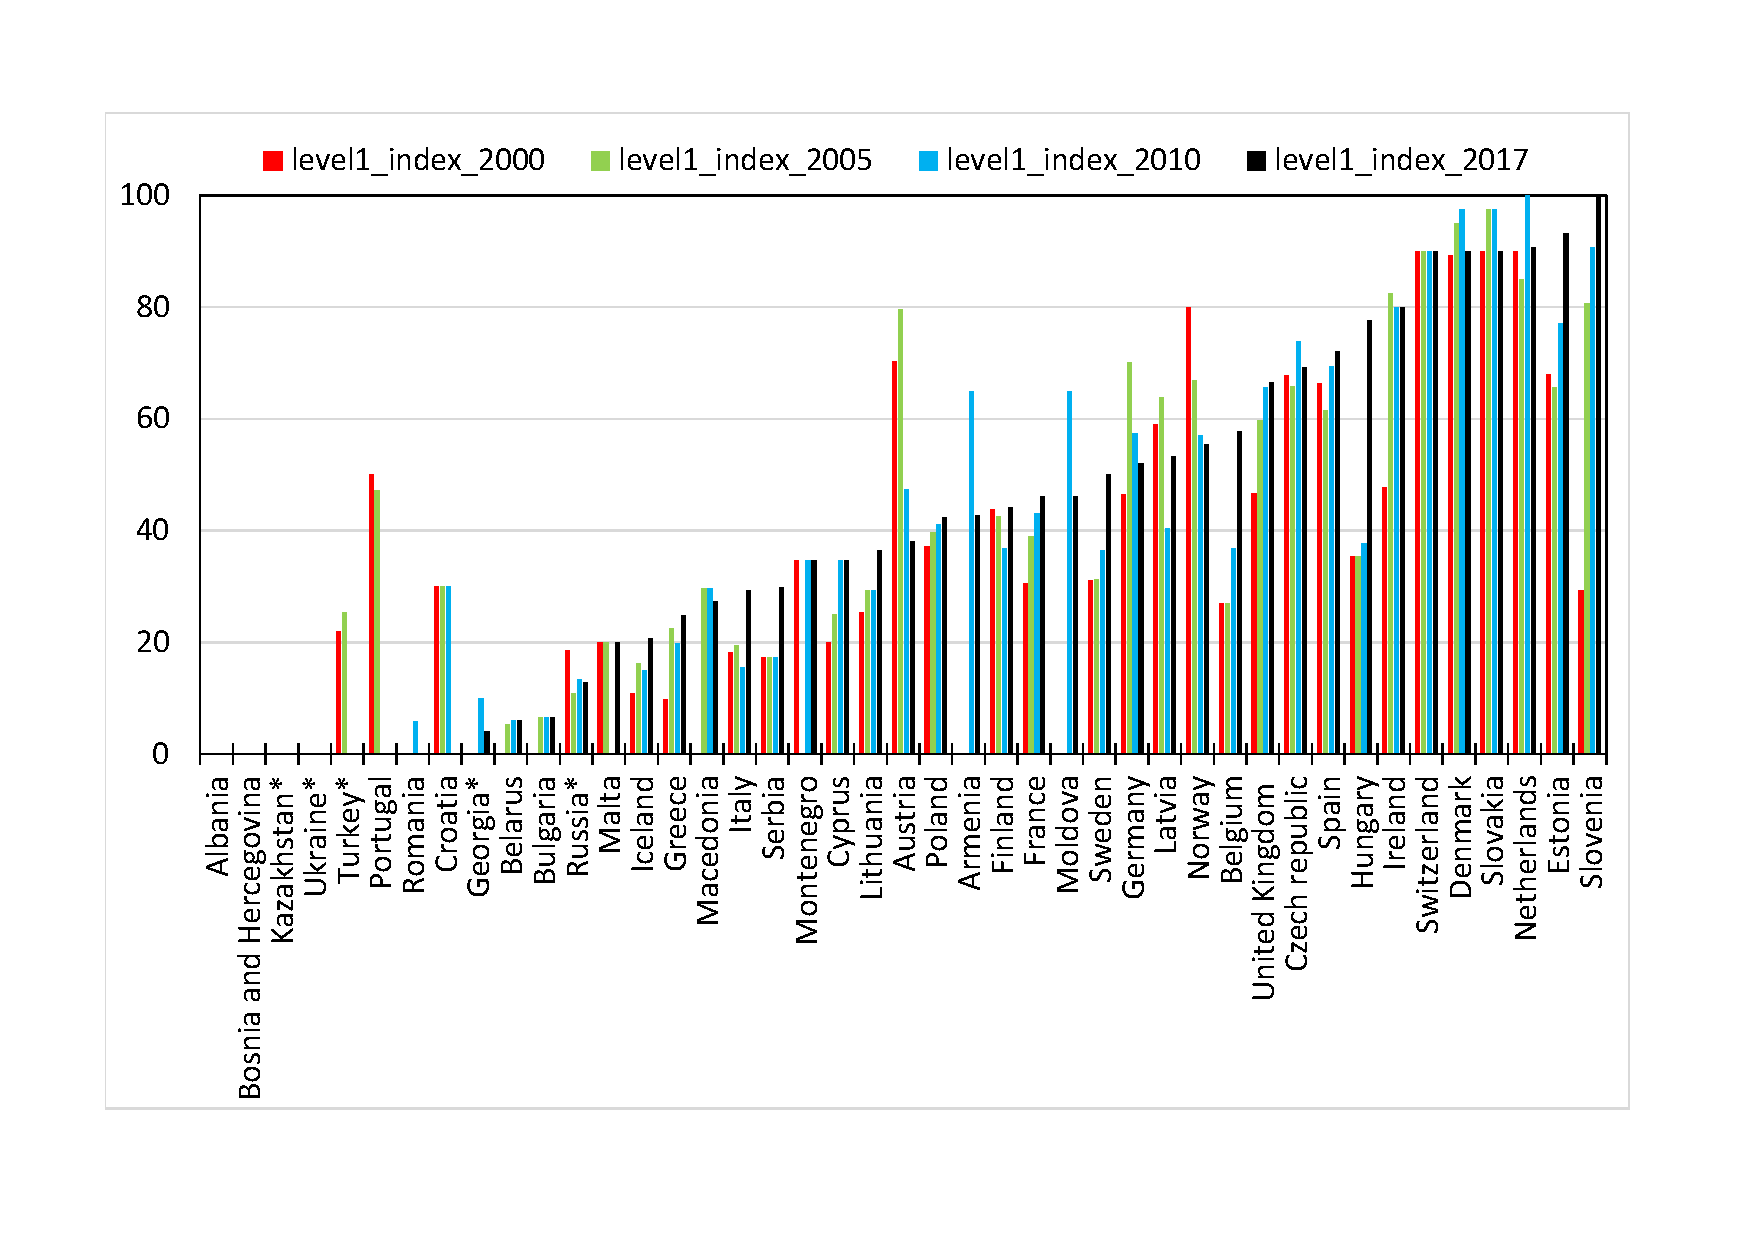
\includegraphics[width=0.74\paperwidth]{FIGS_Obs/index2017.pdf}
	\caption{\label{fig:Index-for-implementation}Index for implementation of the EMEP monitoring strategy, level 1 based on what has been reported for 2000, 2005, 2010 and 2016. {*} means adjusted land area.}
\end{figure}

For the level 2 parameters, an index based system has not been defined, but mapping the site distribution illustrate the 
compliance to the monitoring strategy. 45 sites from 18 different Parties reported  at least one of the required 
EMEP level 2 parameters relevant to this report (aerosols (36 sites), photo-oxidants (19 sites) and trace gases (9 sites)). 
The sites with measurements of POPs and heavy metals are covered in the EMEP status report published by MSC-E. 
Figure~\ref{fig:levell2-sites} shows that level 2 measurements of aerosols have better spatial coverage 
than oxidant precursors (VOC + methane) and trace gases. Few sites have a complete measurement program, 
and only 8 sites have a complete aerosol program. Nevertheless, regarding the aerosol monitoring, 
there have been large improvements in the spatial coverage and the data quality over the last decade. 
Standardization and reference methodologies have been developed, and the reporting has improved significantly 
with much more metadata information available. For oxidant precursors and trace gases, there are ongoing improvement in the measurement capabilities resulting from development in ACTRIS (Aerosols, Clouds, and Trace gases 
Research InfraStructure Network) and in co-operation with the WMO Global Atmospheric Watch Programme (GAW). 




\clearpage
\bibliographystyle{copernicus}         % change bibliography-name after each
\renewcommand\bibname{References}      % bibliographystyle command!
\addcontentsline{toc}{section}{References}
\bibliography{Refs,EMEP_Reports}
